% Mathematical and graphical reference: ../1-practice_activities/G11_T2_L1_C3_practice.tex
% User scope: retain the existing three independent exercises; exactly two tasks per problem.
\makeatletter
\def\input@path{{../../../preamble/}}
\makeatother
\input{preamble.tex}
% Shared highlight dependencies are retained exclusively for appended Solutions.
\input{highlights/highlights.tex}
% \GTenHighlightsfalse % Uncomment to disable instructional highlights.
\HighlightRegistryPalette
\HighlightRegistryRoles
\usepackage{pdflscape}
\usepackage{needspace}
\usepackage{varwidth}

\geometry{letterpaper,margin=0.25in}
\pagestyle{empty}
\linespread{1.04}
\setlength{\parskip}{2pt}
\raggedbottom
\newenvironment{datagrid}[1]{\par\begingroup\small\setlength{\tabcolsep}{4pt}\setlength{\parskip}{0pt}\renewcommand{\arraystretch}{1.03}\tabularx{\linewidth}{#1}\hline}{\endtabularx\par\endgroup}
\pgfplotsset{relation/.style={width=.94\linewidth,height=7.1cm,axis lines=left,
 grid=major,major grid style={black!15},tick label style={font=\small},
 label style={font=\small},scaled ticks=false,enlargelimits=false,clip=true,
 tick label style={/pgf/number format/1000 sep={}}}}
% Reference label format, ordinary grayscale typography, five IDs per graph.
\newcommand{\PointLabel}[7]{%
 \node[font=\small,fill=white,inner sep=1.5pt,anchor=#7] (point#1)
 at (axis description cs:#5,#6) {#1: $(#3,\,#4)$};
 \draw[black!70,line width=.35pt,shorten <=2.5pt] (axis cs:#2)--(point#1);
}
% Scoped to the two linear worked-example panels: equally spaced west
% anchors on y=slope*x+offset, parallel to the normalized data line.
\newcommand{\LinearGuideLabel}[6][south east]{%
 \pgfmathsetmacro{\guideX}{\guideStart+#6*\guideStep}%
 \pgfmathsetmacro{\guideY}{\guideSlope*\guideX+\guideOffset}%
 % Freeze coordinates before pgfplots defers axis-node placement.
 \edef\placeGuide{\noexpand\coordinate (guide#2) at
 (axis description cs:\guideX,\guideY);}\placeGuide
 \node[font=\small,fill=white,inner sep=1pt,anchor=west] (point#2)
 at (guide#2) {#2: $(#4,\,#5)$};
 \draw[black!70,line width=.35pt,shorten <=2.5pt]
 (axis cs:#3)--(point#2.#1);
}
\newcommand{\normalpanel}[2]{%
 \par\noindent\begin{tikzpicture}\begin{axis}[
 width=.80\linewidth,height=1.05cm,scale only axis,
 xmin=-4,xmax=4,ymin=0,ymax=.46,enlargelimits=false,axis lines=left,
 xtick={-#2,0,#2},xticklabels={$-#2$,0,$+#2$},ytick={0,.4},
 tick label style={font=\footnotesize},label style={font=\small},
 title={$C=#1\%\qquad -z^*=-#2,\quad +z^*=+#2$},
 title style={font=\small,yshift=-2pt}]
 \addplot[draw=none,fill=black!18,domain=-#2:#2,samples=161]
 {exp(-x*x/2)/sqrt(2*pi)}\closedcycle;
 \addplot[black,thick,domain=-4:4,samples=201] {exp(-x*x/2)/sqrt(2*pi)};
 \draw[dashed] (axis cs:-#2,0)--(axis cs:-#2,.33)
 (axis cs:#2,0)--(axis cs:#2,.33);
 \node[font=\small] at (axis cs:0,.17) {$#1\%$};
 \end{axis}\end{tikzpicture}\par}
\begin{document}
\newgeometry{margin=0.25in,includefoot,footskip=14pt}
\begingroup % Printable activity only; flush before restoring Solutions settings.
\pagenumbering{arabic}
\pagestyle{plain}
\setlength{\parskip}{1pt}
% Structural styles for the printable activity only; no semantic highlighting.
\newcommand{\stageheading}[1]{%
    \par\Needspace{3\baselineskip}\addvspace{1pt}%
    {\centering\large\bfseries
     \tikz[baseline=(title.base)]{%
         \node[fill=black!10,draw=black,line width=0.2pt,text=black,rounded corners=2mm,
             inner sep=3pt,outer sep=0pt] (title) {\strut #1};}\par}%
    \nopagebreak[4]\vspace{1pt}
}
\newcommand{\criterionbox}[2]{%
    \begin{tcolorbox}[colback=white,colframe=black!45,boxrule=.4pt,
        arc=2mm,boxsep=0pt,left=6pt,right=6pt,top=5pt,bottom=5pt,
        before skip=4pt,after skip=4pt,width=\linewidth]
        \textbf{#1} #2
    \end{tcolorbox}%
}
\newcommand{\problemtitle}[2]{%
    \par\Needspace{3\baselineskip}\noindent\textbf{#1. #2}\par\nopagebreak[4]}
% Level 2: full numbered task title in #1; optional instructions in #2.
% Shade only the title and padding; wrap within the local linewidth.
\newcommand{\taskheading}[1]{%
    \par\Needspace{3\baselineskip}\addvspace{1pt}%
    \noindent\tikz[baseline=(title.base)]{%
        \node[fill=black!5,draw=none,text=black,rounded corners=2mm,
            inner sep=3pt,outer sep=0pt] (title) {%
            \begin{varwidth}{\dimexpr\linewidth-6pt\relax}%
                \raggedright\bfseries\strut #1\strut
            \end{varwidth}};}\par\nopagebreak[4]\vspace{1pt}
}
\newcommand{\task}[2]{\taskheading{#1}#2}
% Level 3: restart 1--3 within each task; instructions stay outside underline.
% Keep titles short: ordinary underline is intentionally unbreakable.
\newcommand{\subtaskheading}[2]{%
    \par\Needspace{3\baselineskip}\addvspace{1pt}%
    \noindent{\color{black}\textbf{\underline{#1. #2.}}}\par
    \nopagebreak[4]\vspace{1pt}
}


{\centering{\Large\bfseries C3: Anatomy of a confidence interval\par}
Global Economics | Grade 11 | Term 2 | Lesson 1\par}
\criterionbox{C3}{Identifies the components of a confidence interval, including point estimate, critical value, standard error, and margin of error, explaining how each component affects precision and reliability.}


\stageheading{Equations and basic procedure}
A confidence interval estimates an unknown population mean $\mu$ and shows the uncertainty around a sample mean. Its width depends on population variability, sample size, and confidence.\par
\begingroup
\small\setlength{\tabcolsep}{3pt}\setlength{\extrarowheight}{0pt}
\setlength{\parskip}{0pt}\renewcommand{\arraystretch}{1}
\begin{tabularx}{\linewidth}{@{}>{\raggedright\arraybackslash}p{.12\linewidth}>{\raggedright\arraybackslash}p{.23\linewidth}>{\raggedright\arraybackslash}X@{}}
\toprule
\textbf{Symbol} & \textbf{Concept} & \textbf{Definition and formula}\\\midrule
$\mathrm{CI}$ & Confidence interval & Range estimating $\mu$: $[\bar{x}-\mathrm{MoE},\bar{x}+\mathrm{MoE}]$; in the measured units.\\
$\bar{x}$ & Point estimate & Sample mean estimating $\mu$; centre of the interval, in the measured units.\\
$C$ & Confidence level & Nominal long-run percentage of intervals covering $\mu$ under the model.\\
$z^*$ & Critical value & Positive standard normal cutoff with central area $C/100$ when $C$ is a percentage; unitless.\\
$\mathrm{SE}$ & Standard error & Standard deviation of sample means: $\mathrm{SE}=\sigma/\sqrt n$; in the measured units.\\
$\mathrm{MoE}$ & Margin of error & Distance from the estimate to either endpoint: $\mathrm{MoE}=z^*\mathrm{SE}$; in the measured units.\\
$\sigma$ & Population standard deviation & Known spread of individual population values; in the measured units.\\
$n$ & Sample size & Number of sampled units; a positive integer count.\\
\bottomrule
\end{tabularx}\par\endgroup

\stageheading{General tasks}
\task{Task 1 -- Investigate SE, MoE, and sample size with $\mathbf{\sigma}$ and confidence fixed.}{}
Calculate SE and MoE for the five sample sizes, assigned A--E in the stated order. Draw (top left) SE vs $n$, (top right) MoE vs $n$, and (bottom left) MoE vs SE. 

\task{Task 2 -- Investigate confidence, critical value, and MoE with $n$ and $\sigma$ fixed.}{}
Calculate the fixed SE and the MoE for each supplied $(C,z^*)$ pair. Draw (top left) confidence vs MoE, (top right) critical value vs MoE, and (bottom left) confidence vs critical value. Use these five cases in every problem:
\begin{datagrid}{|l|X|X|X|X|X|}ID&A&B&C&D&E\\\hline
$C$ (\%)&80&90&95&99&99.9\\\hline
$z^*$&1.282&1.645&1.960&2.576&3.291\\\hline\end{datagrid}

\vspace{2pt}
\textbf{For both tasks.} Plot all five cases in each relationship graph, label A--E with their $(x,y)$ coordinates, and draw the corresponding curve or line. SE and MoE have the context's monetary units; $n$ counts sampled units, $C$ uses percent, and $z^*$ is unitless. The bottom-right cell is calculation workspace in student problems; supplementary illustrations appear only in the worked example.

\pgfplotsset{relation/.append style={height=4.9cm}}
\Needspace{5cm}
\stageheading{Worked example}
\problemtitle{1}{Weekly household grocery spending} 
An analyst estimates the district mean weekly household grocery bill. For the explanatory intervals, the common point estimate is $\bar{x}=84$ thousand COP.
Population SD is known: $\sigma=30$ thousand COP; the common assumptions apply. For Task 1, fix $C=95\%$ ($z^*=1.960$) and use $n=25,100,400,900,1600$ for A--E, respectively. For Task 2, fix $n=100$ and the same $\sigma$, using the five general $(C,z^*)$ cases.
\task{Task 1 -- Investigate SE, MoE, and sample size with $\mathbf{\sigma}$ and confidence fixed.}{}
\subtaskheading{1}{Calculations}
\noindent\begin{minipage}[t]{.30\linewidth}\vspace{0pt}
\textbf{Solution.} For A, $\mathrm{SE}=30/\sqrt{25}=6.000$ and $\mathrm{MoE}=1.960(6.000)=11.760$ thousand COP. The remaining substitutions supply the other plotted coordinates.
\end{minipage}\hfill
\begin{minipage}[t]{.68\linewidth}\vspace{0pt}
\begin{datagrid}{|l|r|X|X|}ID&$n$&SE (thousand COP)&MoE (thousand COP)\\\hline
A&25&$30/\sqrt{25}=6.000$&$1.960(6.000)=11.760$\\\hline
B&100&$30/\sqrt{100}=3.000$&$1.960(3.000)=5.880$\\\hline
C&400&$30/\sqrt{400}=1.500$&$1.960(1.500)=2.940$\\\hline
D&900&$30/\sqrt{900}=1.000$&$1.960(1.000)=1.960$\\\hline
E&1600&$30/\sqrt{1600}=0.750$&$1.960(0.750)=1.470$\\\hline
\end{datagrid}
\end{minipage}\par
\par\smallskip
\Needspace{5.4cm}
\subtaskheading{2}{Relationship graphs}
\begin{minipage}[t]{.49\linewidth}\vspace{0pt}\centering\textbf{Standard error vs sample size}\par\smallskip
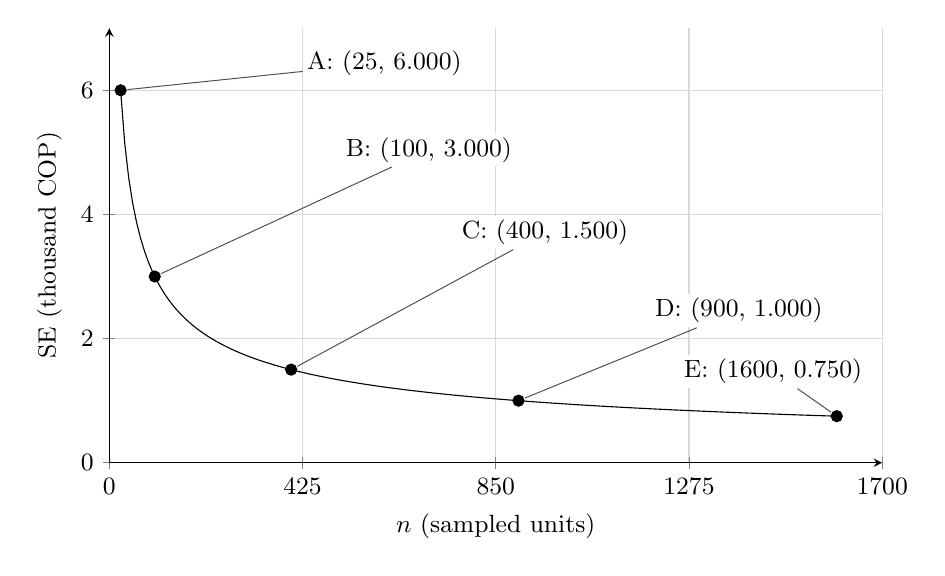
\begin{tikzpicture}\begin{axis}[relation,xlabel={$n$ (sampled units)},ylabel={SE (thousand COP)},xmin=0,xmax=1700,ymin=0,ymax=7,xtick={0,425,850,1275,1700}]
\addplot[black,domain=25:1600,samples=180] {30/sqrt(x)};
\addplot[only marks,mark=*,mark size=2pt] coordinates {(25.000000000,6.000000000) (100.000000000,3.000000000) (400.000000000,1.500000000) (900.000000000,1.000000000) (1600.000000000,0.750000000)};
\PointLabel{A}{25.000000000,6.000000000}{25}{6.000}{0.25}{0.92}{west}
\PointLabel{B}{100.000000000,3.000000000}{100}{3.000}{0.3}{0.72}{west}
\PointLabel{C}{400.000000000,1.500000000}{400}{1.500}{0.45}{0.53}{west}
\PointLabel{D}{900.000000000,1.000000000}{900}{1.000}{0.7}{0.35}{west}
\PointLabel{E}{1600.000000000,0.750000000}{1600}{0.750}{0.98}{0.21}{east}
\end{axis}\end{tikzpicture}\end{minipage}
\hfill
\begin{minipage}[t]{.49\linewidth}\vspace{0pt}\centering\textbf{Margin of error vs sample size}\par\smallskip
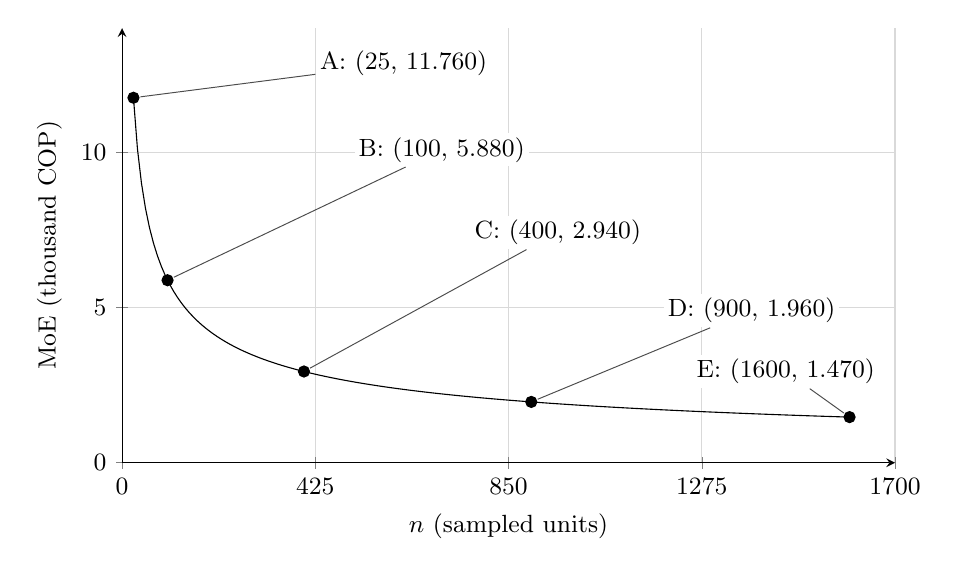
\begin{tikzpicture}\begin{axis}[relation,xlabel={$n$ (sampled units)},ylabel={MoE (thousand COP)},xmin=0,xmax=1700,ymin=0,ymax=14,xtick={0,425,850,1275,1700}]
\addplot[black,domain=25:1600,samples=180] {1.960*30/sqrt(x)};
\addplot[only marks,mark=*,mark size=2pt] coordinates {(25.000000000,11.760000000) (100.000000000,5.880000000) (400.000000000,2.940000000) (900.000000000,1.960000000) (1600.000000000,1.470000000)};
\PointLabel{A}{25.000000000,11.760000000}{25}{11.760}{0.25}{0.92}{west}
\PointLabel{B}{100.000000000,5.880000000}{100}{5.880}{0.3}{0.72}{west}
\PointLabel{C}{400.000000000,2.940000000}{400}{2.940}{0.45}{0.53}{west}
\PointLabel{D}{900.000000000,1.960000000}{900}{1.960}{0.7}{0.35}{west}
\PointLabel{E}{1600.000000000,1.470000000}{1600}{1.470}{0.98}{0.21}{east}
\end{axis}\end{tikzpicture}\end{minipage}
\par\smallskip
\begin{minipage}[t]{.49\linewidth}\vspace{0pt}\centering\textbf{Margin of error vs standard error}\par\smallskip
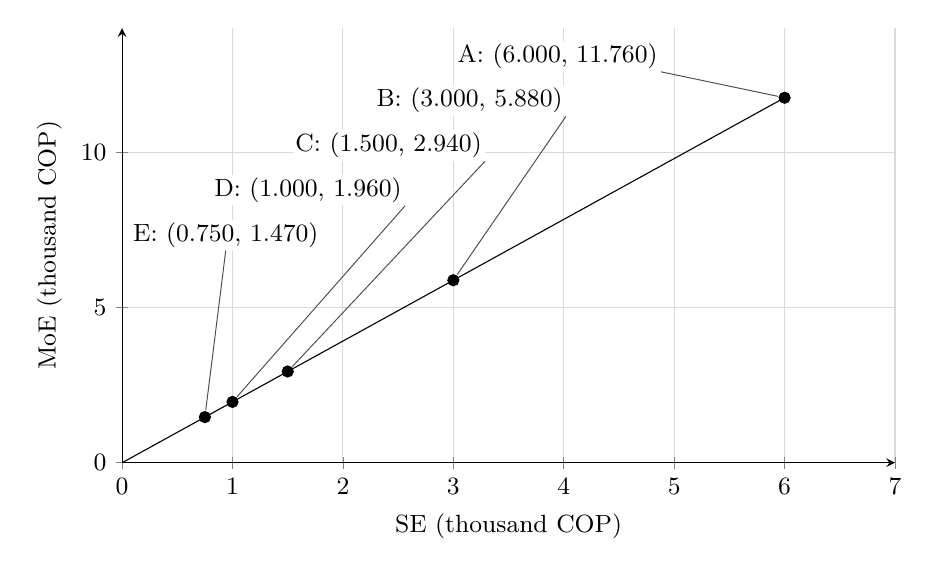
\begin{tikzpicture}\begin{axis}[relation,xlabel={SE (thousand COP)},ylabel={MoE (thousand COP)},xmin=0,xmax=7,ymin=0,ymax=14]
\addplot[black,domain=0:6.0] {1.960*x};
\addplot[only marks,mark=*,mark size=2pt] coordinates {(6.000000000,11.760000000) (3.000000000,5.880000000) (1.500000000,2.940000000) (1.000000000,1.960000000) (0.750000000,1.470000000)};
\def\guideStart{0.010}\def\guideStep{0.105}%
\def\guideSlope{1.960*7/14}\def\guideOffset{0.5147}%
\LinearGuideLabel{A}{6.000000000,11.760000000}{6.000}{11.760}{4}
\LinearGuideLabel{B}{3.000000000,5.880000000}{3.000}{5.880}{3}
\LinearGuideLabel{C}{1.500000000,2.940000000}{1.500}{2.940}{2}
\LinearGuideLabel[south east]{D}{1.000000000,1.960000000}{1.000}{1.960}{1}
\LinearGuideLabel[south]{E}{0.750000000,1.470000000}{0.750}{1.470}{0}
\end{axis}\end{tikzpicture}

SE $\sim$ MoE $\sim$ $1/\sqrt n$. Larger samples give narrower intervals and greater precision at the same 95\% confidence.

\end{minipage}
\hfill\begin{minipage}[t]{.49\linewidth}\vspace{0pt}\small
\textbf{Explanatory confidence-interval comparison}\par
These three intervals use $\bar{x}\pm\mathrm{MoE}=84\pm1.960(30/\sqrt n)$, in 1000 COP:\par
\(\begin{gathered}
\begin{aligned}
n=25:&\quad84\pm11.760=[72.240,95.760],\\
n=400:&\quad84\pm2.940=[81.060,86.940],\\
n=1600:&\quad84\pm1.470=[82.530,85.470].
\end{aligned}
\end{gathered}\)
\centering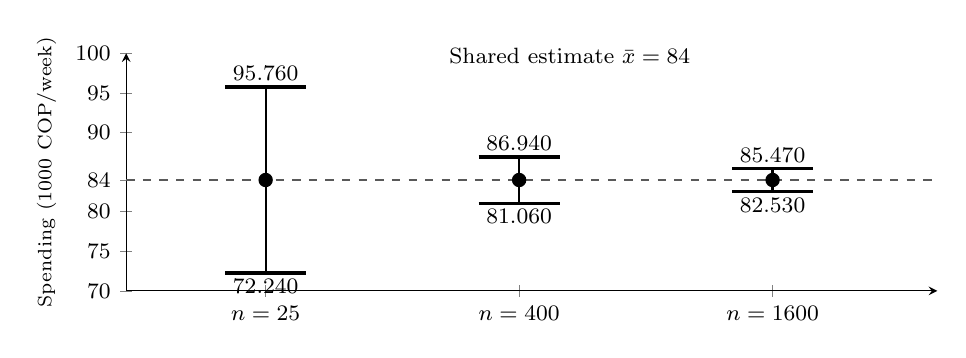
\begin{tikzpicture}\begin{axis}[
width=.98\linewidth,height=4.6cm,xmin=.45,xmax=3.65,ymin=70,ymax=100,
axis x line=bottom,axis y line=left,xtick={1,2,3},
xticklabels={$n=25$,$n=400$,$n=1600$},ytick={70,75,80,84,90,95,100},
tick label style={font=\footnotesize},label style={font=\footnotesize},
ylabel={\scriptsize Spending (1000 COP/week)},scaled ticks=false,clip=false]
\draw[dashed,black!65] (axis cs:.45,84)--(axis cs:3.65,84);
\node[font=\footnotesize,anchor=south] at (axis cs:2.2,97.5) {Shared estimate $\bar{x}=84$};
\draw[thick] (axis cs:1,72.240)--(axis cs:1,95.760);
\draw[line width=1.3pt] (axis cs:0.84,72.240)--(axis cs:1.16,72.240)
(axis cs:0.84,95.760)--(axis cs:1.16,95.760);
\fill (axis cs:1,84) circle (2.6pt);
\node[font=\footnotesize,anchor=north,inner sep=2pt] at (axis cs:1,72.240) {72.240};
\node[font=\footnotesize,anchor=south,inner sep=2pt] at (axis cs:1,95.760) {95.760};
\draw[thick] (axis cs:2,81.060)--(axis cs:2,86.940);
\draw[line width=1.3pt] (axis cs:1.84,81.060)--(axis cs:2.16,81.060)
(axis cs:1.84,86.940)--(axis cs:2.16,86.940);
\fill (axis cs:2,84) circle (2.6pt);
\node[font=\footnotesize,anchor=north,inner sep=2pt] at (axis cs:2,81.060) {81.060};
\node[font=\footnotesize,anchor=south,inner sep=2pt] at (axis cs:2,86.940) {86.940};
\draw[thick] (axis cs:3,82.530)--(axis cs:3,85.470);
\draw[line width=1.3pt] (axis cs:2.84,82.530)--(axis cs:3.16,82.530)
(axis cs:2.84,85.470)--(axis cs:3.16,85.470);
\fill (axis cs:3,84) circle (2.6pt);
\node[font=\footnotesize,anchor=north,inner sep=2pt] at (axis cs:3,82.530) {82.530};
\node[font=\footnotesize,anchor=south,inner sep=2pt] at (axis cs:3,85.470) {85.470};
\end{axis}\end{tikzpicture}\par
\end{minipage}\par

\vspace{2pt}

\Needspace{3cm}
\task{Task 2  -- Investigate confidence, critical value, and MoE with $n$ and $\sigma$ fixed.}{Use $n=100$}
\subtaskheading{1}{Calculations}
\textbf{Solution.} $\mathrm{SE}=30/\sqrt{100}=3.000$ thousand COP. Thus the five margins are $1.282(3)=3.846$, $1.645(3)=4.935$, $1.960(3)=5.880$, $2.576(3)=7.728$ and $3.291(3)=9.873$ thousand COP.
\par\smallskip
\Needspace{5.4cm}
\subtaskheading{2}{Relationship graphs}
\begin{minipage}[t]{.49\linewidth}\vspace{0pt}\centering\textbf{Confidence level vs margin of error}\par\smallskip
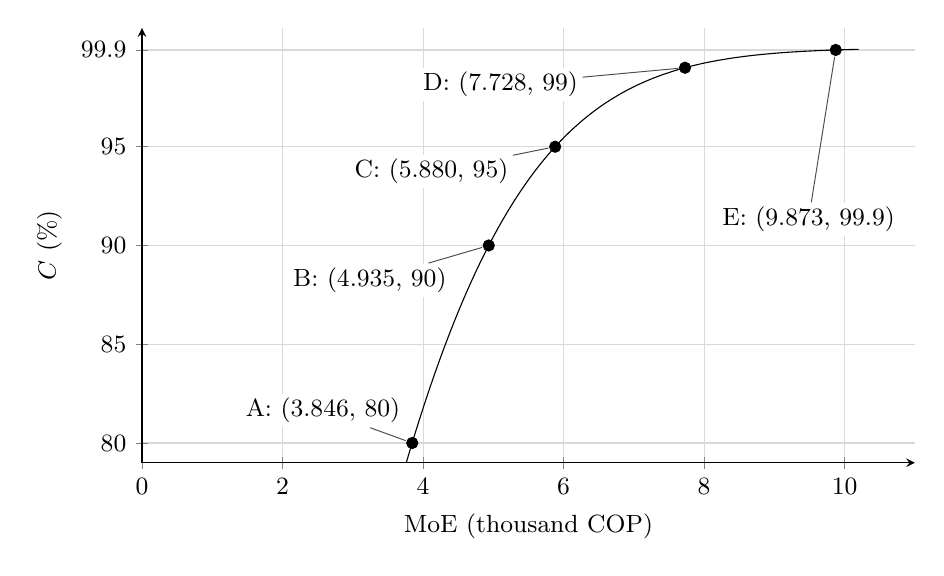
\begin{tikzpicture}\begin{axis}[relation,xlabel={MoE (thousand COP)},ylabel={$C$ (\%)},xmin=0,xmax=11,ymin=79,ymax=101,ytick={80,85,90,95,99.9}]
\addplot[black] coordinates {(3.600000000,76.986065956) (3.636666667,77.457267281) (3.673333333,77.921538814) (3.710000000,78.378914140) (3.746666667,78.829428390) (3.783333333,79.273118204) (3.820000000,79.710021689) (3.856666667,80.140178381) (3.893333333,80.563629207) (3.930000000,80.980416441) (3.966666667,81.390583669) (4.003333333,81.794175746) (4.040000000,82.191238757) (4.076666667,82.581819974) (4.113333333,82.965967820) (4.150000000,83.343731826) (4.186666667,83.715162592) (4.223333333,84.080311743) (4.260000000,84.439231895) (4.296666667,84.791976609) (4.333333333,85.138600354) (4.370000000,85.479158469) (4.406666667,85.813707116) (4.443333333,86.142303250) (4.480000000,86.465004571) (4.516666667,86.781869494) (4.553333333,87.092957100) (4.590000000,87.398327107) (4.626666667,87.698039826) (4.663333333,87.992156125) (4.700000000,88.280737392) (4.736666667,88.563845498) (4.773333333,88.841542760) (4.810000000,89.113891904) (4.846666667,89.380956033) (4.883333333,89.642798585) (4.920000000,89.899483305) (4.956666667,90.151074208) (4.993333333,90.397635545) (5.030000000,90.639231769) (5.066666667,90.875927504) (5.103333333,91.107787513) (5.140000000,91.334876665) (5.176666667,91.557259905) (5.213333333,91.775002224) (5.250000000,91.988168627) (5.286666667,92.196824108) (5.323333333,92.401033617) (5.360000000,92.600862035) (5.396666667,92.796374145) (5.433333333,92.987634608) (5.470000000,93.174707932) (5.506666667,93.357658453) (5.543333333,93.536550307) (5.580000000,93.711447404) (5.616666667,93.882413408) (5.653333333,94.049511715) (5.690000000,94.212805427) (5.726666667,94.372357332) (5.763333333,94.528229888) (5.800000000,94.680485196) (5.836666667,94.829184985) (5.873333333,94.974390591) (5.910000000,95.116162944) (5.946666667,95.254562542) (5.983333333,95.389649443) (6.020000000,95.521483244) (6.056666667,95.650123066) (6.093333333,95.775627542) (6.130000000,95.898054799) (6.166666667,96.017462450) (6.203333333,96.133907575) (6.240000000,96.247446713) (6.276666667,96.358135850) (6.313333333,96.466030405) (6.350000000,96.571185226) (6.386666667,96.673654573) (6.423333333,96.773492113) (6.460000000,96.870750912) (6.496666667,96.965483425) (6.533333333,97.057741490) (6.570000000,97.147576318) (6.606666667,97.235038493) (6.643333333,97.320177959) (6.680000000,97.403044022) (6.716666667,97.483685338) (6.753333333,97.562149914) (6.790000000,97.638485104) (6.826666667,97.712737601) (6.863333333,97.784953441) (6.900000000,97.855177996) (6.936666667,97.923455973) (6.973333333,97.989831414) (7.010000000,98.054347695) (7.046666667,98.117047523) (7.083333333,98.177972938) (7.120000000,98.237165314) (7.156666667,98.294665358) (7.193333333,98.350513110) (7.230000000,98.404747948) (7.266666667,98.457408586) (7.303333333,98.508533080) (7.340000000,98.558158826) (7.376666667,98.606322564) (7.413333333,98.653060386) (7.450000000,98.698407731) (7.486666667,98.742399394) (7.523333333,98.785069530) (7.560000000,98.826451657) (7.596666667,98.866578658) (7.633333333,98.905482789) (7.670000000,98.943195683) (7.706666667,98.979748356) (7.743333333,99.015171209) (7.780000000,99.049494036) (7.816666667,99.082746030) (7.853333333,99.114955789) (7.890000000,99.146151318) (7.926666667,99.176360042) (7.963333333,99.205608807) (8.000000000,99.233923886) (8.036666667,99.261330993) (8.073333333,99.287855279) (8.110000000,99.313521347) (8.146666667,99.338353257) (8.183333333,99.362374529) (8.220000000,99.385608156) (8.256666667,99.408076609) (8.293333333,99.429801841) (8.330000000,99.450805300) (8.366666667,99.471107932) (8.403333333,99.490730189) (8.440000000,99.509692041) (8.476666667,99.528012976) (8.513333333,99.545712013) (8.550000000,99.562807709) (8.586666667,99.579318164) (8.623333333,99.595261032) (8.660000000,99.610653524) (8.696666667,99.625512422) (8.733333333,99.639854079) (8.770000000,99.653694435) (8.806666667,99.667049015) (8.843333333,99.679932946) (8.880000000,99.692360958) (8.916666667,99.704347393) (8.953333333,99.715906214) (8.990000000,99.727051011) (9.026666667,99.737795010) (9.063333333,99.748151076) (9.100000000,99.758131727) (9.136666667,99.767749133) (9.173333333,99.777015132) (9.210000000,99.785941229) (9.246666667,99.794538609) (9.283333333,99.802818141) (9.320000000,99.810790383) (9.356666667,99.818465596) (9.393333333,99.825853741) (9.430000000,99.832964493) (9.466666667,99.839807245) (9.503333333,99.846391114) (9.540000000,99.852724948) (9.576666667,99.858817332) (9.613333333,99.864676596) (9.650000000,99.870310818) (9.686666667,99.875727832) (9.723333333,99.880935234) (9.760000000,99.885940387) (9.796666667,99.890750427) (9.833333333,99.895372271) (9.870000000,99.899812617) (9.906666667,99.904077957) (9.943333333,99.908174575) (9.980000000,99.912108558) (10.016666667,99.915885798) (10.053333333,99.919511999) (10.090000000,99.922992681) (10.126666667,99.926333183) (10.163333333,99.929538672) (10.200000000,99.932614147)};
\addplot[only marks,mark=*,mark size=2pt] coordinates {(3.846000000,80.000000000) (4.935000000,90.000000000) (5.880000000,95.000000000) (7.728000000,99.000000000) (9.873000000,99.900000000)};
\PointLabel{A}{3.846000000,80.000000000}{3.846}{80}{0.34}{0.12}{east}
\PointLabel{B}{4.935000000,90.000000000}{4.935}{90}{0.40}{0.42}{east}
\PointLabel{C}{5.880000000,95.000000000}{5.880}{95}{0.48}{0.67}{east}
\PointLabel{D}{7.728000000,99.000000000}{7.728}{99}{0.57}{0.87}{east}
\PointLabel{E}{9.873000000,99.900000000}{9.873}{99.9}{0.98}{0.56}{east}
\end{axis}\end{tikzpicture}\end{minipage}
\hfill
\begin{minipage}[t]{.49\linewidth}\vspace{0pt}\centering\textbf{Critical value vs margin of error}\par\smallskip
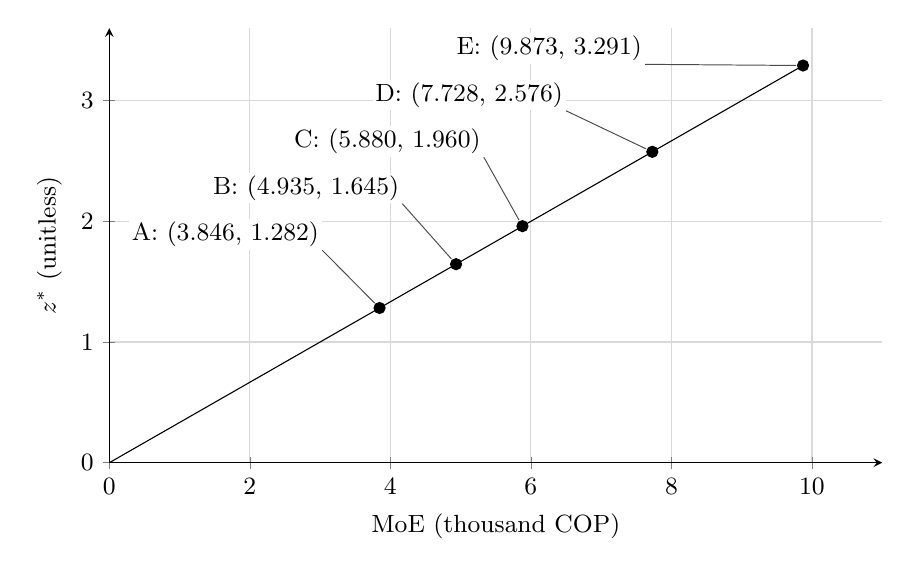
\begin{tikzpicture}\begin{axis}[relation,xlabel={MoE (thousand COP)},ylabel={$z^*$ (unitless)},xmin=0,xmax=11,ymin=0,ymax=3.6,ytick={0,1,2,3}]
\addplot[black,domain=0:9.873] {x/3.0};
\addplot[only marks,mark=*,mark size=2pt] coordinates {(3.846000000,1.282000000) (4.935000000,1.645000000) (5.880000000,1.960000000) (7.728000000,2.576000000) (9.873000000,3.291000000)};
\def\guideStart{0.025}\def\guideStep{0.105}%
\def\guideSlope{11/(3*3.6)}\def\guideOffset{0.50}%
\LinearGuideLabel{A}{3.846000000,1.282000000}{3.846}{1.282}{0}
\LinearGuideLabel{B}{4.935000000,1.645000000}{4.935}{1.645}{1}
\LinearGuideLabel{C}{5.880000000,1.960000000}{5.880}{1.960}{2}
\LinearGuideLabel{D}{7.728000000,2.576000000}{7.728}{2.576}{3}
\LinearGuideLabel{E}{9.873000000,3.291000000}{9.873}{3.291}{4}
\end{axis}\end{tikzpicture}\end{minipage}
\par\smallskip
\begin{minipage}[t]{.49\linewidth}\vspace{0pt}\centering\textbf{Confidence level vs critical value}\par\smallskip
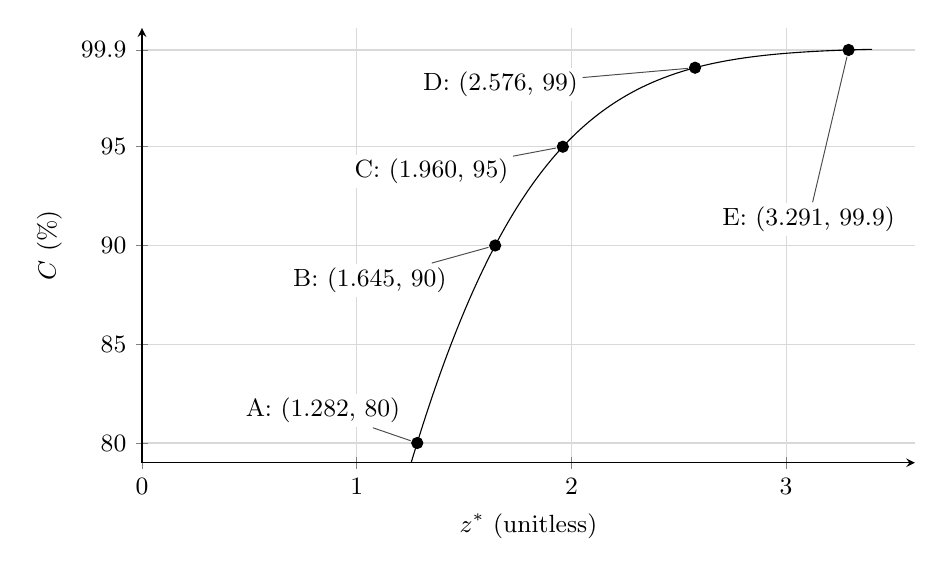
\begin{tikzpicture}\begin{axis}[relation,xlabel={$z^*$ (unitless)},ylabel={$C$ (\%)},xmin=0,xmax=3.6,ymin=79,ymax=101,xtick={0,1,2,3},ytick={80,85,90,95,99.9}]
\addplot[black] coordinates {(1.200000000,76.986065956) (1.212222222,77.457267281) (1.224444444,77.921538814) (1.236666667,78.378914140) (1.248888889,78.829428390) (1.261111111,79.273118204) (1.273333333,79.710021689) (1.285555556,80.140178381) (1.297777778,80.563629207) (1.310000000,80.980416441) (1.322222222,81.390583669) (1.334444444,81.794175746) (1.346666667,82.191238757) (1.358888889,82.581819974) (1.371111111,82.965967820) (1.383333333,83.343731826) (1.395555556,83.715162592) (1.407777778,84.080311743) (1.420000000,84.439231895) (1.432222222,84.791976609) (1.444444444,85.138600354) (1.456666667,85.479158469) (1.468888889,85.813707116) (1.481111111,86.142303250) (1.493333333,86.465004571) (1.505555556,86.781869494) (1.517777778,87.092957100) (1.530000000,87.398327107) (1.542222222,87.698039826) (1.554444444,87.992156125) (1.566666667,88.280737392) (1.578888889,88.563845498) (1.591111111,88.841542760) (1.603333333,89.113891904) (1.615555556,89.380956033) (1.627777778,89.642798585) (1.640000000,89.899483305) (1.652222222,90.151074208) (1.664444444,90.397635545) (1.676666667,90.639231769) (1.688888889,90.875927504) (1.701111111,91.107787513) (1.713333333,91.334876665) (1.725555556,91.557259905) (1.737777778,91.775002224) (1.750000000,91.988168627) (1.762222222,92.196824108) (1.774444444,92.401033617) (1.786666667,92.600862035) (1.798888889,92.796374145) (1.811111111,92.987634608) (1.823333333,93.174707932) (1.835555556,93.357658453) (1.847777778,93.536550307) (1.860000000,93.711447404) (1.872222222,93.882413408) (1.884444444,94.049511715) (1.896666667,94.212805427) (1.908888889,94.372357332) (1.921111111,94.528229888) (1.933333333,94.680485196) (1.945555556,94.829184985) (1.957777778,94.974390591) (1.970000000,95.116162944) (1.982222222,95.254562542) (1.994444444,95.389649443) (2.006666667,95.521483244) (2.018888889,95.650123066) (2.031111111,95.775627542) (2.043333333,95.898054799) (2.055555556,96.017462450) (2.067777778,96.133907575) (2.080000000,96.247446713) (2.092222222,96.358135850) (2.104444444,96.466030405) (2.116666667,96.571185226) (2.128888889,96.673654573) (2.141111111,96.773492113) (2.153333333,96.870750912) (2.165555556,96.965483425) (2.177777778,97.057741490) (2.190000000,97.147576318) (2.202222222,97.235038493) (2.214444444,97.320177959) (2.226666667,97.403044022) (2.238888889,97.483685338) (2.251111111,97.562149914) (2.263333333,97.638485104) (2.275555556,97.712737601) (2.287777778,97.784953441) (2.300000000,97.855177996) (2.312222222,97.923455973) (2.324444444,97.989831414) (2.336666667,98.054347695) (2.348888889,98.117047523) (2.361111111,98.177972938) (2.373333333,98.237165314) (2.385555556,98.294665358) (2.397777778,98.350513110) (2.410000000,98.404747948) (2.422222222,98.457408586) (2.434444444,98.508533080) (2.446666667,98.558158826) (2.458888889,98.606322564) (2.471111111,98.653060386) (2.483333333,98.698407731) (2.495555556,98.742399394) (2.507777778,98.785069530) (2.520000000,98.826451657) (2.532222222,98.866578658) (2.544444444,98.905482789) (2.556666667,98.943195683) (2.568888889,98.979748356) (2.581111111,99.015171209) (2.593333333,99.049494036) (2.605555556,99.082746030) (2.617777778,99.114955789) (2.630000000,99.146151318) (2.642222222,99.176360042) (2.654444444,99.205608807) (2.666666667,99.233923886) (2.678888889,99.261330993) (2.691111111,99.287855279) (2.703333333,99.313521347) (2.715555556,99.338353257) (2.727777778,99.362374529) (2.740000000,99.385608156) (2.752222222,99.408076609) (2.764444444,99.429801841) (2.776666667,99.450805300) (2.788888889,99.471107932) (2.801111111,99.490730189) (2.813333333,99.509692041) (2.825555556,99.528012976) (2.837777778,99.545712013) (2.850000000,99.562807709) (2.862222222,99.579318164) (2.874444444,99.595261032) (2.886666667,99.610653524) (2.898888889,99.625512422) (2.911111111,99.639854079) (2.923333333,99.653694435) (2.935555556,99.667049015) (2.947777778,99.679932946) (2.960000000,99.692360958) (2.972222222,99.704347393) (2.984444444,99.715906214) (2.996666667,99.727051011) (3.008888889,99.737795010) (3.021111111,99.748151076) (3.033333333,99.758131727) (3.045555556,99.767749133) (3.057777778,99.777015132) (3.070000000,99.785941229) (3.082222222,99.794538609) (3.094444444,99.802818141) (3.106666667,99.810790383) (3.118888889,99.818465596) (3.131111111,99.825853741) (3.143333333,99.832964493) (3.155555556,99.839807245) (3.167777778,99.846391114) (3.180000000,99.852724948) (3.192222222,99.858817332) (3.204444444,99.864676596) (3.216666667,99.870310818) (3.228888889,99.875727832) (3.241111111,99.880935234) (3.253333333,99.885940387) (3.265555556,99.890750427) (3.277777778,99.895372271) (3.290000000,99.899812617) (3.302222222,99.904077957) (3.314444444,99.908174575) (3.326666667,99.912108558) (3.338888889,99.915885798) (3.351111111,99.919511999) (3.363333333,99.922992681) (3.375555556,99.926333183) (3.387777778,99.929538672) (3.400000000,99.932614147)};
\addplot[only marks,mark=*,mark size=2pt] coordinates {(1.282000000,80.000000000) (1.645000000,90.000000000) (1.960000000,95.000000000) (2.576000000,99.000000000) (3.291000000,99.900000000)};
\PointLabel{A}{1.282000000,80.000000000}{1.282}{80}{0.34}{0.12}{east}
\PointLabel{B}{1.645000000,90.000000000}{1.645}{90}{0.40}{0.42}{east}
\PointLabel{C}{1.960000000,95.000000000}{1.960}{95}{0.48}{0.67}{east}
\PointLabel{D}{2.576000000,99.000000000}{2.576}{99}{0.57}{0.87}{east}
\PointLabel{E}{3.291000000,99.900000000}{3.291}{99.9}{0.98}{0.56}{east}
\end{axis}\end{tikzpicture}

At fixed SE, MoE increases with $z^*$. Higher confidence requires a larger $z^*$, producing wider intervals and lower precision. 

\end{minipage}
\hfill\begin{minipage}[t]{.49\linewidth}\vspace{0pt}\centering
\textbf{Explanatory standard normal illustrations}\par
\normalpanel{80}{1.282}\normalpanel{95}{1.960}\normalpanel{99.9}{3.291}
{\small $z$ (unitless); vertical axis: density.\par}
\end{minipage}\par

\pgfplotsset{relation/.append style={height=6.1cm}}
\par
\begingroup % Guided response helpers cannot affect other sections or Solutions.
\newcommand{\guidedresponsebox}[2][9mm]{%
    \tikz[baseline=(answer.base)]{%
        \node[fill=black!1,draw=black!25,line width=.3pt,
            rounded corners=2mm,inner sep=0pt,outer sep=.3pt,
            minimum width=#2,minimum height=#1] (answer) {\phantom{0}};}}
\newcommand{\LabelTemplates}{%
  \node[anchor=east,font=\small,fill=white,inner sep=1.5pt]
    at (axis description cs:.97,.92)
    {A: $(\guidedresponsebox[6mm]{14mm},\,\guidedresponsebox[6mm]{14mm})$};
  \node[anchor=east,font=\small,fill=white,inner sep=1.5pt]
    at (axis description cs:.97,.71)
    {B: $(\guidedresponsebox[6mm]{14mm},\,\guidedresponsebox[6mm]{14mm})$};
  \node[anchor=east,font=\small,fill=white,inner sep=1.5pt]
    at (axis description cs:.97,.50)
    {C: $(\guidedresponsebox[6mm]{14mm},\,\guidedresponsebox[6mm]{14mm})$};
  \node[anchor=east,font=\small,fill=white,inner sep=1.5pt]
    at (axis description cs:.97,.29)
    {D: $(\guidedresponsebox[6mm]{14mm},\,\guidedresponsebox[6mm]{14mm})$};
  \node[anchor=east,font=\small,fill=white,inner sep=1.5pt]
    at (axis description cs:.97,.08)
    {E: $(\guidedresponsebox[6mm]{14mm},\,\guidedresponsebox[6mm]{14mm})$};
}
\newcommand{\workarea}{\begin{minipage}[t]{.49\linewidth}\vspace{0pt}
  \textbf{Calculation workspace}\par\smallskip
  \noindent\guidedresponsebox[4.5cm]{\dimexpr\linewidth-1pt\relax}
  \end{minipage}}
\pgfplotsset{relation/.append style={height=5.1cm}}
\stageheading{Guided Example}
\problemtitle{2}{Delivery charges for local businesses}
A business association estimates the mean charge for a local delivery.
Population SD is known: $\sigma=24$ thousand COP; the common assumptions apply. For Task 1, fix $C=95\%$ ($z^*=1.960$) and use $n=36,100,225,400,900$ for A--E, respectively. For Task 2, fix $n=100$ and the same $\sigma$, using the five general $(C,z^*)$ cases.
\task{Task 1:}{Apply general Task 1 to the five sample sizes above.}
\Needspace{5.5cm}
\subtaskheading{1}{Relationship graphs}
\par
\begin{minipage}[t]{.49\linewidth}\vspace{0pt}\centering\textbf{Standard error vs sample size}\par\smallskip
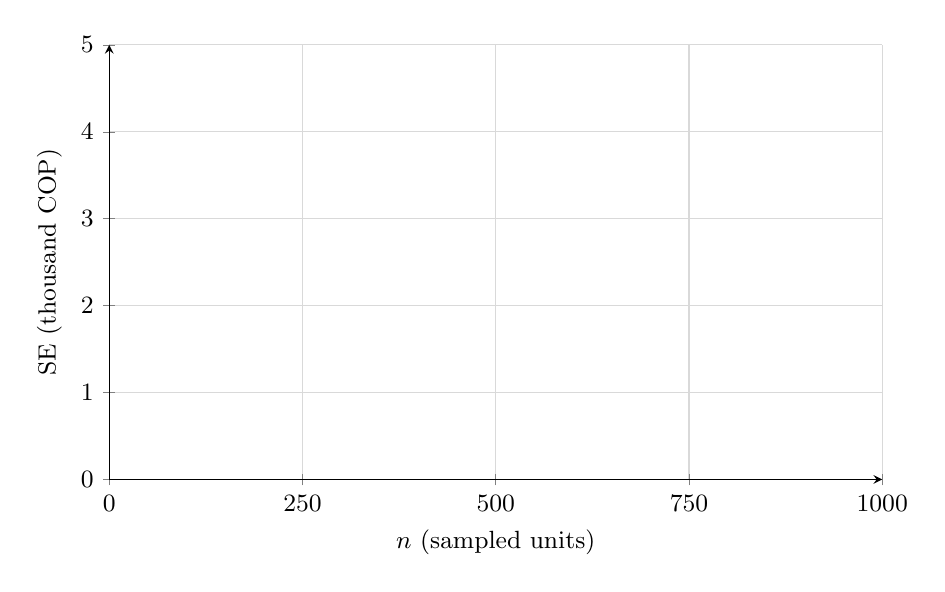
\begin{tikzpicture}\begin{axis}[relation,xlabel={$n$ (sampled units)},ylabel={SE (thousand COP)},xmin=0,xmax=1000,ymin=0,ymax=5,xtick={0,250,500,750,1000}]
\LabelTemplates
\end{axis}\end{tikzpicture}\end{minipage}
\hfill
\begin{minipage}[t]{.49\linewidth}\vspace{0pt}\centering\textbf{Margin of error vs sample size}\par\smallskip
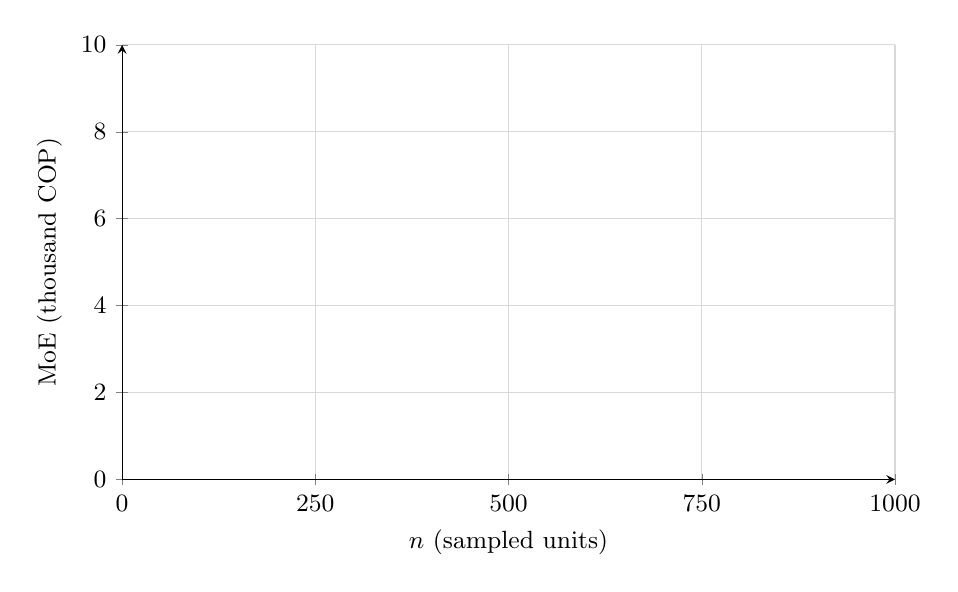
\begin{tikzpicture}\begin{axis}[relation,xlabel={$n$ (sampled units)},ylabel={MoE (thousand COP)},xmin=0,xmax=1000,ymin=0,ymax=10,xtick={0,250,500,750,1000}]
\LabelTemplates
\end{axis}\end{tikzpicture}\end{minipage}
\par\smallskip
\Needspace{5.5cm}
\subtaskheading{2}{Relationship graph and calculations}
\noindent\begin{minipage}[t]{.49\linewidth}\vspace{0pt}\centering\textbf{Margin of error vs standard error}\par\smallskip
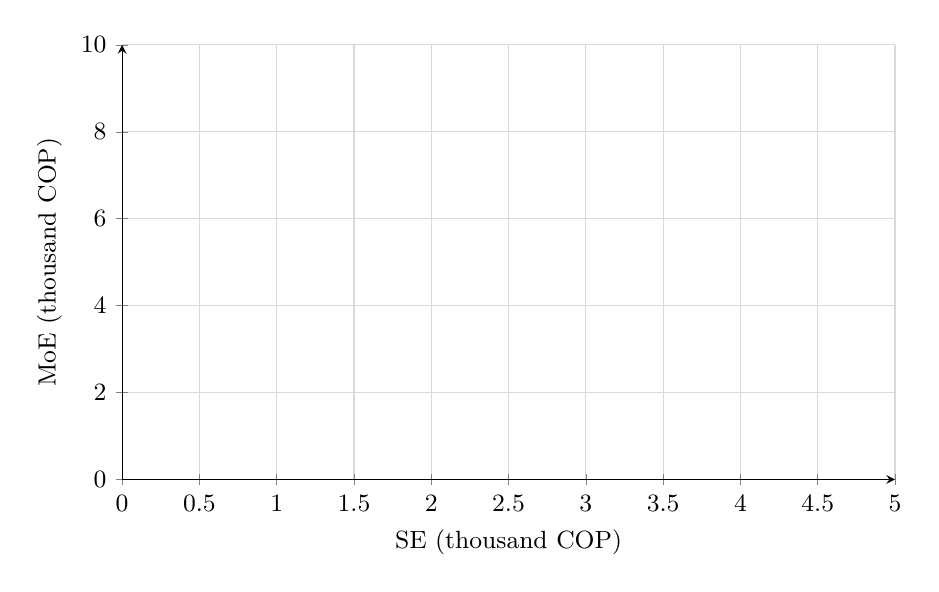
\begin{tikzpicture}\begin{axis}[relation,xlabel={SE (thousand COP)},ylabel={MoE (thousand COP)},xmin=0,xmax=5,ymin=0,ymax=10]
\LabelTemplates
\end{axis}\end{tikzpicture}\end{minipage}
\hfill\workarea\par

\par

\Needspace{7cm}
\textbf{Problem 2 --- Delivery charges for local businesses continued}
\task{Task 2:}{Apply general Task 2 with $n=100$ and the five general confidence cases.}
\Needspace{5.5cm}
\subtaskheading{1}{Relationship graphs}
\par\smallskip
\begin{minipage}[t]{.49\linewidth}\vspace{0pt}\centering\textbf{Confidence level vs margin of error}\par\smallskip
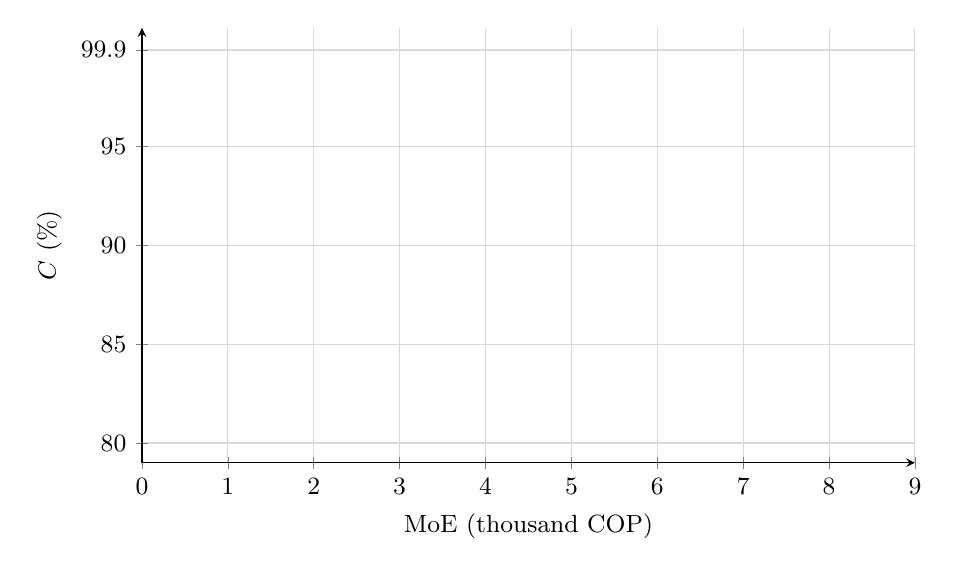
\begin{tikzpicture}\begin{axis}[relation,xlabel={MoE (thousand COP)},ylabel={$C$ (\%)},xmin=0,xmax=9,ymin=79,ymax=101,ytick={80,85,90,95,99.9}]
\LabelTemplates
\end{axis}\end{tikzpicture}\end{minipage}
\hfill
\begin{minipage}[t]{.49\linewidth}\vspace{0pt}\centering\textbf{Critical value vs margin of error}\par\smallskip
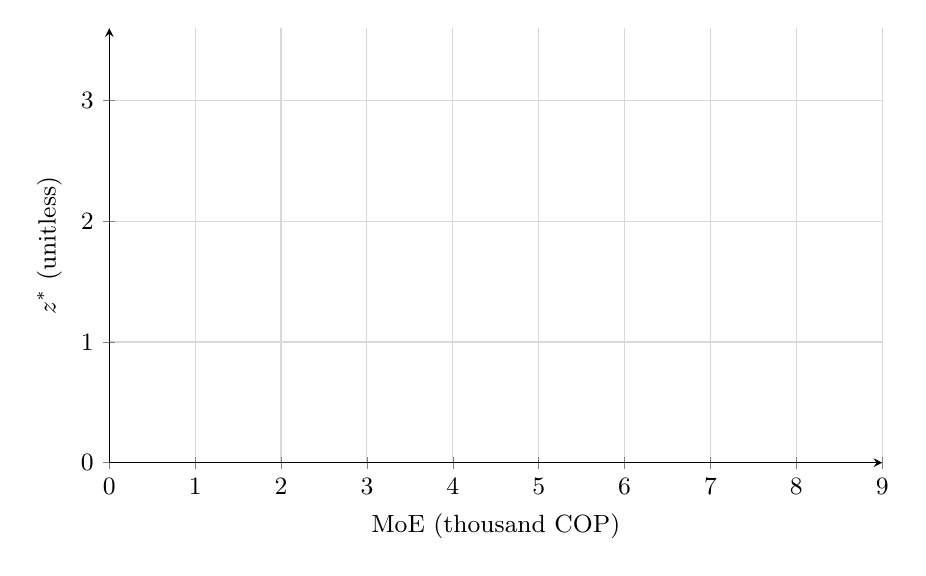
\begin{tikzpicture}\begin{axis}[relation,xlabel={MoE (thousand COP)},ylabel={$z^*$ (unitless)},xmin=0,xmax=9,ymin=0,ymax=3.6,ytick={0,1,2,3}]
\LabelTemplates
\end{axis}\end{tikzpicture}\end{minipage}
\par\smallskip
\Needspace{5.5cm}
\subtaskheading{2}{Relationship graph and calculations}
\noindent\begin{minipage}[t]{.49\linewidth}\vspace{0pt}\centering\textbf{Confidence level vs critical value}\par\smallskip
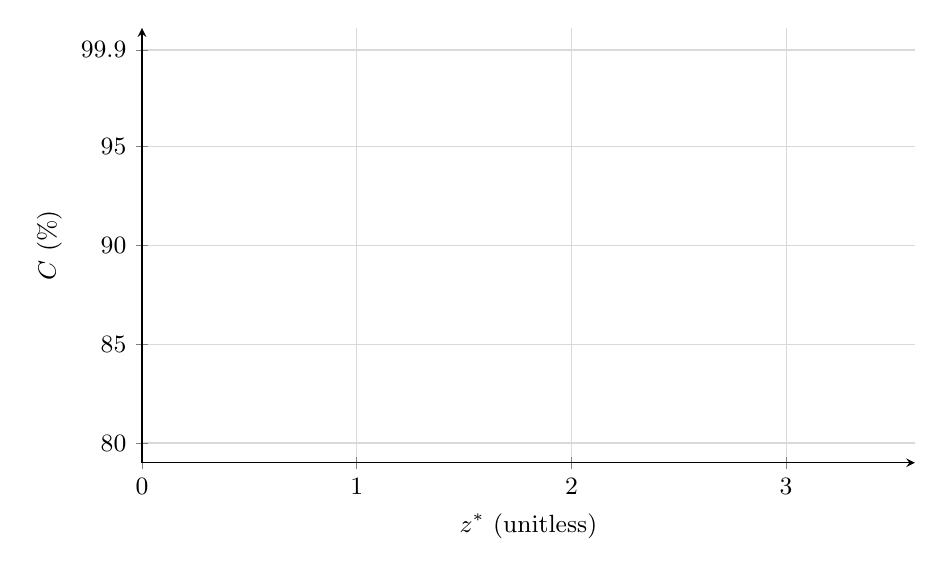
\begin{tikzpicture}\begin{axis}[relation,xlabel={$z^*$ (unitless)},ylabel={$C$ (\%)},xmin=0,xmax=3.6,ymin=79,ymax=101,xtick={0,1,2,3},ytick={80,85,90,95,99.9}]
\LabelTemplates
\end{axis}\end{tikzpicture}\end{minipage}
\hfill\workarea\par

\par
\endgroup % Guided Example: no page settings changed; activity flush follows below.

\stageheading{Independent Practice}
\begingroup\small\setlength{\parskip}{0pt}
% Run short task titles into their instructions within the independent columns.
% Keep the same compact node and route every title through \taskheading.
\renewcommand{\taskheading}[1]{%
    \par\Needspace{2\baselineskip}\addvspace{1pt}%
    \noindent\tikz[baseline=(title.base)]{%
        \node[fill=black!5,draw=none,text=black,rounded corners=2mm,
            inner sep=3pt,outer sep=0pt] (title) {%
            \begin{varwidth}{\dimexpr\linewidth-6pt\relax}%
                \raggedright\bfseries\strut #1\strut
            \end{varwidth}};}\nobreak\hspace{3pt}}
\textit{Complete Independent Practice on a separate sheet.}\par

\noindent\begin{minipage}[t]{.325\linewidth}\vspace{0pt}\raggedright
\problemtitle{3}{Weekly market-stall revenue}
A market office estimates mean weekly revenue per stall.
Population SD is known: $\sigma=45$ thousand COP; the common assumptions apply. For Task 1, fix $C=95\%$ ($z^*=1.960$) and use $n=25,100,225,625,1600$ for A--E, respectively. For Task 2, fix $n=225$ and the same $\sigma$, using the five general $(C,z^*)$ cases.
\task{Task 1:}{Calculate SE and MoE for cases A--E. Graph SE vs $n$, MoE vs $n$, and MoE vs SE, labelling all five cases with their coordinates and drawing the corresponding curves or lines.}

\task{Task 2:}{For the five general $(C,z^*)$ cases, calculate SE and MoE. Graph confidence vs MoE, critical value vs MoE, and confidence vs critical value, labelling all five cases with their coordinates and drawing the corresponding curves or lines.}

\end{minipage}\hfill
\begin{minipage}[t]{.325\linewidth}\vspace{0pt}\raggedright
\problemtitle{4}{Freight handling fees}
A port analyst estimates the mean handling fee per container.
Population SD is known: $\sigma=72$ USD; the common assumptions apply. For Task 1, fix $C=95\%$ ($z^*=1.960$) and use $n=36,144,324,576,1296$ for A--E, respectively. For Task 2, fix $n=144$ and the same $\sigma$, using the five general $(C,z^*)$ cases.
\task{Task 1:}{Calculate SE and MoE for cases A--E. Graph SE vs $n$, MoE vs $n$, and MoE vs SE, labelling all five cases with their coordinates and drawing the corresponding curves or lines.}

\task{Task 2:}{For the five general $(C,z^*)$ cases, calculate SE and MoE. Graph confidence vs MoE, critical value vs MoE, and confidence vs critical value, labelling all five cases with their coordinates and drawing the corresponding curves or lines.}

\end{minipage}\hfill
\begin{minipage}[t]{.325\linewidth}\vspace{0pt}\raggedright
\problemtitle{5}{Monthly internet costs}
A district estimates mean monthly internet expenditure per small business.
Population SD is known: $\sigma=35$ thousand COP; the common assumptions apply. For Task 1, fix $C=95\%$ ($z^*=1.960$) and use $n=49,100,196,400,1225$ for A--E, respectively. For Task 2, fix $n=196$ and the same $\sigma$, using the five general $(C,z^*)$ cases.
\task{Task 1:}{Calculate SE and MoE for cases A--E. Graph SE vs $n$, MoE vs $n$, and MoE vs SE, labelling all five cases with their coordinates and drawing the corresponding curves or lines.}

\task{Task 2:}{For the five general $(C,z^*)$ cases, calculate SE and MoE. Graph confidence vs MoE, critical value vs MoE, and confidence vs critical value, labelling all five cases with their coordinates and drawing the corresponding curves or lines.}
\end{minipage}
\par\endgroup
\par\clearpage
\endgroup
\end{document}